\newpage
\hypertarget{rules vis}{}
\subsection{Visual Rules}
\visHeader

Some sort of content so that we don't start right away with a subsection. In essence, this section wants to create a rule normally, and then DERIVE a second
one. In the second rule, we should do 'create new correspondence type' in the window, to show users they don't HAVE to include it in the schema before using
(declare it on the fly.. not have to switch diagram). maybe in this paragraph we can explain how we'll meet the TGG goals (producitivy, maintability, etc etc))

\subsection{BoxToDictionaryRule}
\begin{enumerate}
\item[$\blacktriangleright$] In EA, open the \texttt{Rules} diagram of your TGG project, automatically generated when you first created it. This diagram must
contain any rules relevant to this project.

\item[$\blacktriangleright$] Create your first rule by either holding \texttt{ctrl} while you click in the diagram, or drag-and-drop the \texttt{Rule} item from
the TGG toolbox to the left of the diagram window (Fig.~\ref{fig:create_tgg_rule}). Now press \texttt{alt + enter} to raise its \texttt{Properties} dialogue.
Update its name to \texttt{BoxToDictionaryRule}.

\vspace{0.5cm}

\begin{figure}[htbp]
\begin{center}
  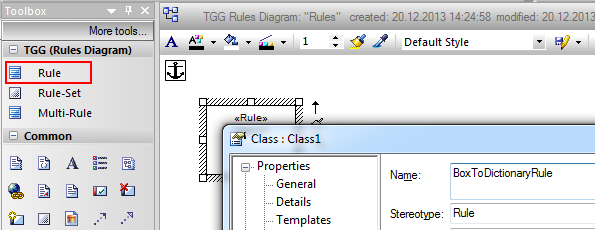
\includegraphics[width=\textwidth]{ea_TGGNewRule}
  \caption{Creating a TGG rule}
  \label{fig:create_tgg_rule}
\end{center}
\end{figure}

\item[$\blacktriangleright$] Double click the element to open the \texttt{BoxToDictionaryRule} diagram. Drag-and-drop the \texttt{Box EClass} from the project
browser into the diagram, choosing to paste the element as an instance from the drop-down menu.\footnote{If the 'Paste Element' dialogue doesn't appear, hold
\texttt{ctrl} and confirm you haven't autosaved the choice as the default move in the \texttt{options} drop-down menu.} The \texttt{name} and \texttt{binding
operator} should already be set to \texttt{box} and \texttt{create}.

\item[$\blacktriangleright$] Repeat the action to create an instance of \texttt{Dictionary}.

\item[$\blacktriangleright$] Quick-link from \texttt{box} to \texttt{dictionary} and create a TGG Correspondence link. To keep things simple, name it
\texttt{boxToDictionary} and select the correspondence type from the drop-down list, which you declared in the schema.

Believe it or not, our rule \emph{already} creates a \texttt{Box}, \texttt{Dictionary}, and correspondence link between them at the same time, as-is!
Unfortunately, this only creates the objects, and doesn't relate any of there values. Why don't we try to connect the \texttt{name} of the \texttt{box} to the \texttt{title}
of the dictionary? I.e., if you have a \texttt{Kitten} LearningBox, you can transform it into a \texttt{Kitten} Dictionary. Luckily, we can once again use
\emph{attribute constraints}!\footnote{These were first defined in Part III, Section 4}. When used with TGG rules, attribute constraints provide a bidirectional
and high-level solution for attribute manipulation. We're looking for a constraint which ensures that \texttt{box.name} and \texttt{dictionary.title} are
consistent

\item[$\blacktriangleright$] Following the same process as a new \texttt{Rule}, either hold \texttt{ctrl} and click in the diagram
(Fig.~\ref{fig:common_toolbox}), or drag-and-drop a \emph{TGG Constraint} from the \texttt{TGGRuleTolboxPage} to create a constraint.

\begin{figure}[htbp]
\begin{center}
  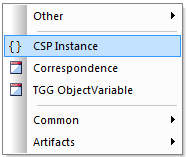
\includegraphics[width=0.3\textwidth]{ea_createTGGConstraint}
  \caption{Constraint from the Toolbox in EA}
  \label{fig:common_toolbox}
\end{center}
\end{figure}

\item[$\blacktriangleright$] Double click the empty box to open its \texttt{TGGConstraint Dialog}. There's a pre-populated list of available constraints; Choose
\texttt{eq} and double click each of the \texttt{Value} fields to specify the \texttt{a} and \texttt{b} values as depicted in
Fig.~\ref{fig:first_tgg_constraint}. Add the constraint and affirm with \texttt{OK}.

\item[$\blacktriangleright$] Your rule should now resemble Fig.~\ref{fig:tgg_rule_with_constraint}, where the new links represent the dependencies between the
  constrain and objects involved

\newpage

\begin{figure}[htbp]
\begin{center}
  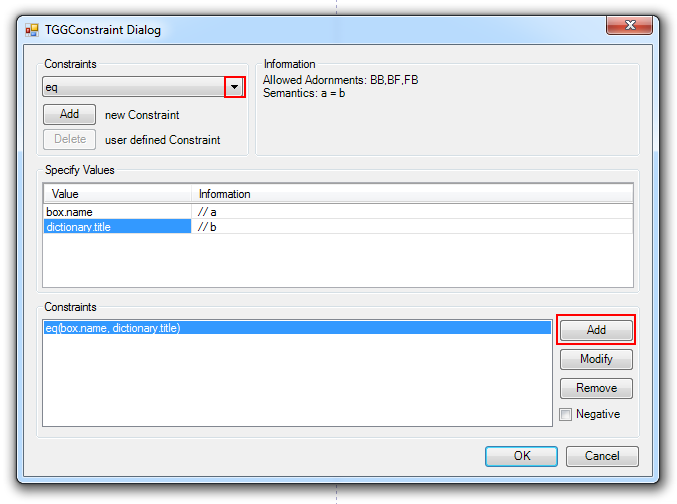
\includegraphics[width=\textwidth]{ea_TGGConstraintDialog}
  \caption{Creating a Constraint in EA}
  \label{fig:first_tgg_constraint}
\end{center}
\end{figure}

\begin{figure}[h!]
\begin{center}
  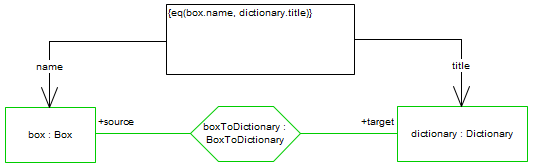
\includegraphics[width=\textwidth]{ea_TGGconstraintDependency}
  \caption{A TGG Rule with a Constraint}
  \label{fig:tgg_rule_with_constraint}
  \end{center}
\end{figure}

\newpage

Our first TGG Rule is not yet complete -- we still need to create the initial structure of learning box. In contrast to the rather
simple dictionary, where \texttt{Dictionary} is a direct container for \texttt{Entry} objects, we have to create a number of connected \texttt{Partitions} that hold
the \texttt{Cards} in the learning box. 

\item[$\blacktriangleright$] Create three \texttt{Partition} object variables, with appropriate link variables that satisfy the LeitnerBoxRules (the
\texttt{next}, \texttt{previous}, and \texttt{box} references). Your TGG rule should then closely resemble Fig.~\ref{fig:boxtodictionaryrule_complete}.


\begin{figure}[htbp]
\begin{center}
  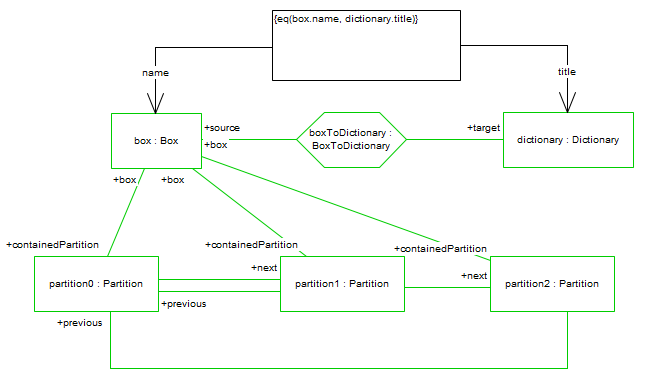
\includegraphics[width=1.1\textwidth]{ea_TGGCompleteRule}
  \caption{Complete TGG rule diagram for \texttt{BoxToDictionaryRule}}
  \label{fig:boxtodictionaryrule_complete}
\end{center}
\end{figure}

\end{enumerate}

% SECOND RULE BEGINS

If you are in hurry, you can jump ahead and proceed to Section~\ref{sect:TGGs_in_Action}: TGGs in Action and transform a box to a dictionary and vice-versa, but
please be aware that your specified TGG (with just one rule) will only be able to cope with empty boxes and dictionaries. Handling additional elements
(i.e., cards in the learning box and entries in the dictionary) requires a second rule. We intend to create this next.

\newpage
\subsection{CardToEntryRule}

Do you remember our \emph{productivity} goal that we hoped to meet with TGGs? Given one rule, we wanted to be able to derive related rules relatively easily.
Luckily, eMoflon is able to do exactly that! To create the rule to take care of \texttt{card}s and \texttt{entry} objects, we can use a cool derivation
feature.

\begin{enumerate}
  
\item[$\blacktriangleright$] First confirm that your eMoflon control panel window is open. If not, activate it by going to ``Extensions/Add-In Windows.''
  
\item[$\blacktriangleright$] Hold \texttt{ctrl} and select each \texttt{box}, \texttt{boxToDictionary}, \texttt{dictionary} and
\texttt{partition0} in the \texttt{Box\-To\-Dictionary\-Rule} diagram.
  
\item[$\blacktriangleright$] Switch to the \texttt{eMoflon TGG Functions} tab on the control panel then press \texttt{Derive} as depicted in
Fig.~\ref{fig:derive_from_tgg_rule}. In the dialogue that appears, enter \texttt{CardToEntryRule} as the name of the rule, and press \texttt{OK.} The new rule
will automatically display in a the editor window.

\begin{figure}[htbp]
\begin{center}
 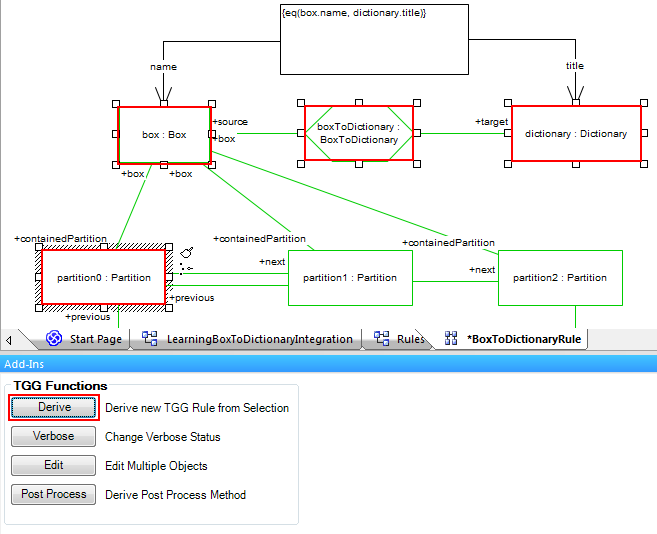
\includegraphics[width=\textwidth]{ea_selectPreDerivation}
  \caption{Derive from an existing TGG rule}
  \label{fig:derive_from_tgg_rule}
\end{center}
\end{figure}
\FloatBarrier

\item[$\blacktriangleright$] Add instances of \texttt{Card} and \texttt{Entry} to the rule and required links until the diagram closely resembles
Fig.~\ref{fig:cardtoentry_1}.

  \begin{figure}[htbp]
  \begin{center}
    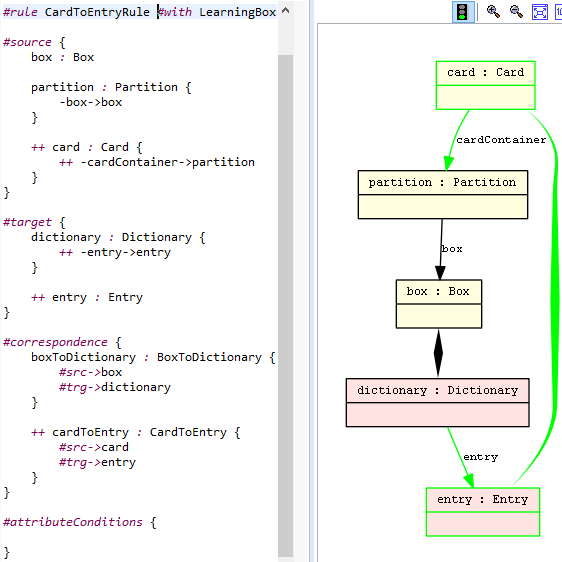
\includegraphics[width=\textwidth]{ea_cardToEntryRule}
    \caption{\texttt{CardToEntryRule} without attribute manipulation}
    \label{fig:cardtoentry_1}
  \end{center}
  \end{figure}

\end{enumerate}

As a final step, we now have to specify how attributes are to be handled via appropriate attribute constraints.

The \texttt{content} of an \texttt{Entry} in a \texttt{Dictionary} is to be of the form \texttt{<word>:<meaning>}, while the \texttt{face} of a \texttt{Card}
must read \texttt{Question:<word>}, and the \texttt{back} of the Card \texttt{Answer:<meaning>}.

Using two predefined attribute constraints, \texttt{addPrefix} and \texttt{concat}, we can specify this as a set of constraints:

\begin{enumerate}
 % Describe the dictionary class? Don't know reasoning behind these variables..
\item[$\blacktriangleright$] Double-click your constraint element and add an \texttt{addPrefix} constraint, where \texttt{prefix} is \texttt{``Question:''},
\texttt{a} is \texttt{word}, and \texttt{b} is \texttt{card.face}.
  
\item[$\blacktriangleright$] Create a second \texttt{addPrefix} constraint with \texttt{``Answer''}, \texttt{meaning}, \texttt{card.back}.

\item[$\blacktriangleright$] Finally, add a \texttt{concat} constraint, with \texttt{``~:~''} as the \texttt{separator}, and \texttt{word}, \texttt{meaning},
\texttt{entry.content} as \texttt{a}, \texttt{b}, \texttt{c}.

\item[$\blacktriangleright$] Your rule should now resemble Fig.~\ref{fig:cardtoentry_2}.

\begin{figure}[htbp]
\begin{center}
  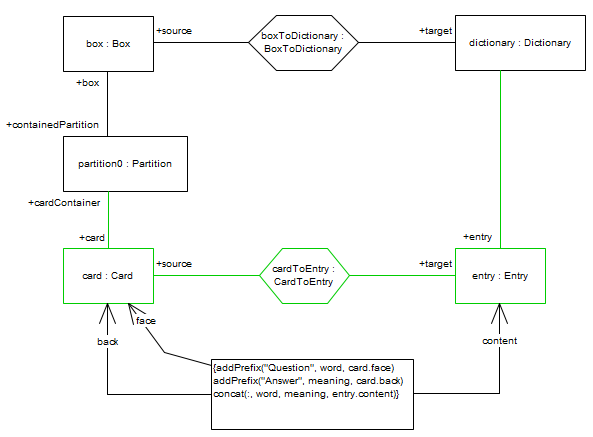
\includegraphics[width=\textwidth]{ea_completedCardToEntry}
  \caption{Attribute manipulation for \texttt{card} and \texttt{entry}}
  \label{fig:cardtoentry_2}
\end{center}
\end{figure}
\FloatBarrier
\end{enumerate}

% Rewrite to make this a bit more clear..
Finally, we have to specify how the partition (into which the new \texttt{card} is to be placed) must be chosen.
We shall implement the following rule: a card in a partition with index 0/1/2 corresponds to an \texttt{Entry} of level beginner/advanced/master.
This time, we must define a unique attribute constraint to handle this mapping. For now, we are just going to declare and use the attribute constraint, which
will be implemented later in Java.

\begin{enumerate}
\item[$\blacktriangleright$] Add one more constraint to your diagram. When you open the dialogue, don't choose a predefined constraint, but instead click
``Add'' below the dropdown menu. Enter the values given in Fig. \ref{fig:create_new_constraint}.

\vspace{0.5cm}

\begin{figure}[htbp]
\begin{center}
  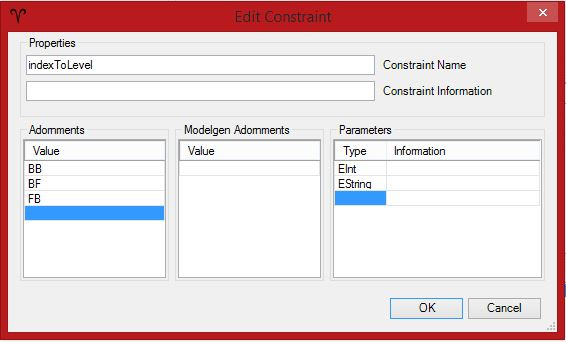
\includegraphics[width=\textwidth]{ea_uniqueConstraint}
  \caption{Create a user defined constraint.}
  \label{fig:create_new_constraint}
\end{center}
\end{figure}
\FloatBarrier

\item[$\blacktriangleright$] Saving this new constraint, then select it from the drop down menu and enter \texttt{partition0.index} as \texttt{Integer} and
\texttt{entry.level} as the \texttt{String}.
\end{enumerate}

After defining the dependencies of the constraint, your complete TGG rule should resemble Fig.~\ref{fig:cardtoentry_complete}.

\newpage

\begin{figure}[htbp]
\begin{center}
  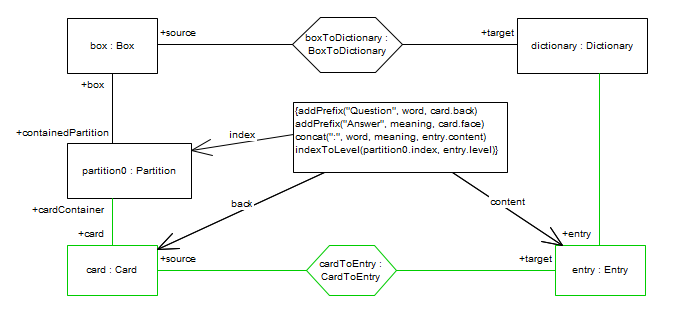
\includegraphics[width=1.2\textwidth]{ea_cardToEntryComplete}
  \caption{\texttt{CardToEntryRule} with complete attribute manipulation}
  \label{fig:cardtoentry_complete}
\end{center}
\end{figure}


